%!TEX root = ..\main.tex
\section{Results}
\subsection{Simulation details}
\label{subsec:simulation_details}

Defining $\rho = \frac{N D}{L}$ where $N$ --- number of particles and $D = \Delta z_{min}$ --- particle diameter, we immediately obtain the simulation system size $L = N D/ \rho$. In our simulations we considered three cases of different densities $\rho = (0.25,\ 0.5,\ 0.95)$.

\textcolor{red}{diameter calculated numerically minimized function. Should I explain it? Not analytically because I'm better with computer than math. And I calculate it every run to get system size}

\textcolor{yellow}{it seems that you need to solve a transcendental equation to obtain the minimum. Thus, you have no way to get it analytically, i.e., the equation cannot be inverted.}

\textcolor{red}{So what should I write here, if at all?}

To check for existence of finite-size effects, for each value of density we perform simulations with different particle numbers $N = (500,\ 5000)$. \textcolor{red}{I've already said that I do it for different density, should I say that I do it for different size instead?}

The Monte-Carlo simulations were allowed to equilibrate for $\Delta = 10^5$ sweeps (one sweep consists of $N$ Monte-Carlo test steps), and after that every $\Delta$ sweeps were generated ensemble-averaged quantities, obtaining $10$ uncorrelated samples.

%\begin{figure}[t]
%	\centering
%	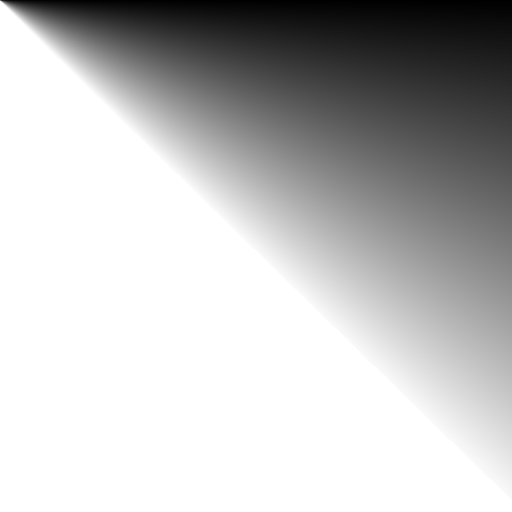
\includegraphics[width=0.5\textwidth, height=0.3\textwidth]{Images/dummy.png}
%	\captionsetup{justification=centering, width=0.9\columnwidth}
%	\caption{Order parameter defined by eq.~\eqref{eq:nematic_order_parameter} versus Monte-Carlo test steps taken by system for different $\epsilon^*$ and $N$}
%	\label{fig:nematic_op_vs_MC_cycles}
%\end{figure}

We measured the following quantities:

Nematic order parameter $S$ is defined as:
\begin{equation}
\label{eq:nematic_order_parameter}
	S = \frac{3 \langle\cos^2 \theta\rangle - 1}{2}
\end{equation}
where $\theta$ it the angle between particle dipole moment and spatial axis, while angle brackets denotes ensemble average.

We also measured the orientation correlation as a function of the distance between particles:
\begin{equation}
	C(\Delta z) = \langle\cos \theta_1 \cos \theta_2\rangle \propto |\Delta z|
\end{equation}
where $\theta_1$ and $\theta_2$ are angles between spatial axis and dipole moments of particles which centers are separated by $\Delta z$ distance. \textcolor{red}{I do it average over some $\Delta z +/- \delta$ area. If I'll just write "separated by $\Delta z +/- \delta$ --- will it be clear?}

We measure the average chain length, where chain is a sequence of chained particles and two particles considered to be "chained" if 
\textcolor{red}{maybe here should be something about energy threshold, plus $<d$ maybe better to be $<d + \delta$?}
\begin{equation}
\begin{cases}
	|z_1 - z_2| &\leq d \\
	\cos \theta_1 \cdot \cos \theta_2 &\geq 0
\end{cases}
\end{equation}